\RequirePackage[hyphens]{url}
\documentclass[11pt,titlepage,dvipsnames,table,xcdraw]{article}
\usepackage{strath-dissertation}
\usepackage{setspace}

\usepackage{babel}
\usepackage{lipsum} % For demonstration only.

% packages specific to this document
\usepackage{pdfpages}
\usepackage{pdflscape}
\usepackage{glossaries}
\usepackage[automake]{glossaries-extra}

% import glossary into preamble
\makeglossaries
\loadglsentries{sections/glossary}

%--------------------------------
% Degree settings
%--------------------------------
\newcommand{\degreename}{Bachelor of Science}
\newcommand{\coursename}{CS408: Individual Project}
\newcommand{\deptname}{Computer and Information Sciences}

\begin{document}

%--------------------------------
% Title page.
%--------------------------------
\begin{titlepage}
\vspace*{5mm}
\titletext{Insert dissertation title here, using\\ manual line breaks if necessary}
\vspace{10mm}
\authortext{A Student}
\vspace{15mm}
\degreetext{\degreename}{\coursename}
\vspace{40mm}
\centredcrest
\vspace{5mm}
\depttext{\deptname}
\vspace{5mm}
\datetext{August, 2021}
\end{titlepage}

%--------------------------------
% Front matter numbering.
%--------------------------------
\pagenumbering{roman}
\setcounter{page}{2}

%--------------------------------
% Setting counter depth.
%--------------------------------
\setcounter{secnumdepth}{3}
\setcounter{tocdepth}{2}

%--------------------------------
% The front matter.
%--------------------------------
\setstretch{1.2} % 1.5 line spacing. 

%Abstract
%Acknowledgements
%Glossary

%    Introduction
%    Background Literature
%    Specification & Design
%    Implementation
%    Evaluation
%    Results
%    Discussion & Reflection
%    Future Work
%    Conclusion

%References
%Appendices


\begin{abstract}
Despite attempts to improve the screen reader accessibility of \latexspaced through \lualatex , frequent use of the outdated \pdflatexspaced leads to many invalid workarounds for accessibility and a web of misinformation found online. With considerations towards appropriate resources, this project identified suitable areas in which screen reader-focused accessibility could be improved in a \latexspaced document.

\lintexspaced achieves this by identifying lacking aspects of screen reader-focused accessibility features in \latexspaced documents and suggesting solutions, often in the form of \gls{tagging} and \gls{image_desc} implementations, that minimise the impact on the end user.

A user study was conducted that identified overall success with \lintexspaced meeting its targets of improving the accessibility of a \latexspaced document for screen reader users and being a generally accessible and maintainable tool.
\end{abstract}
\clearpage

% display overview diagram as full page
\begin{landscape}
	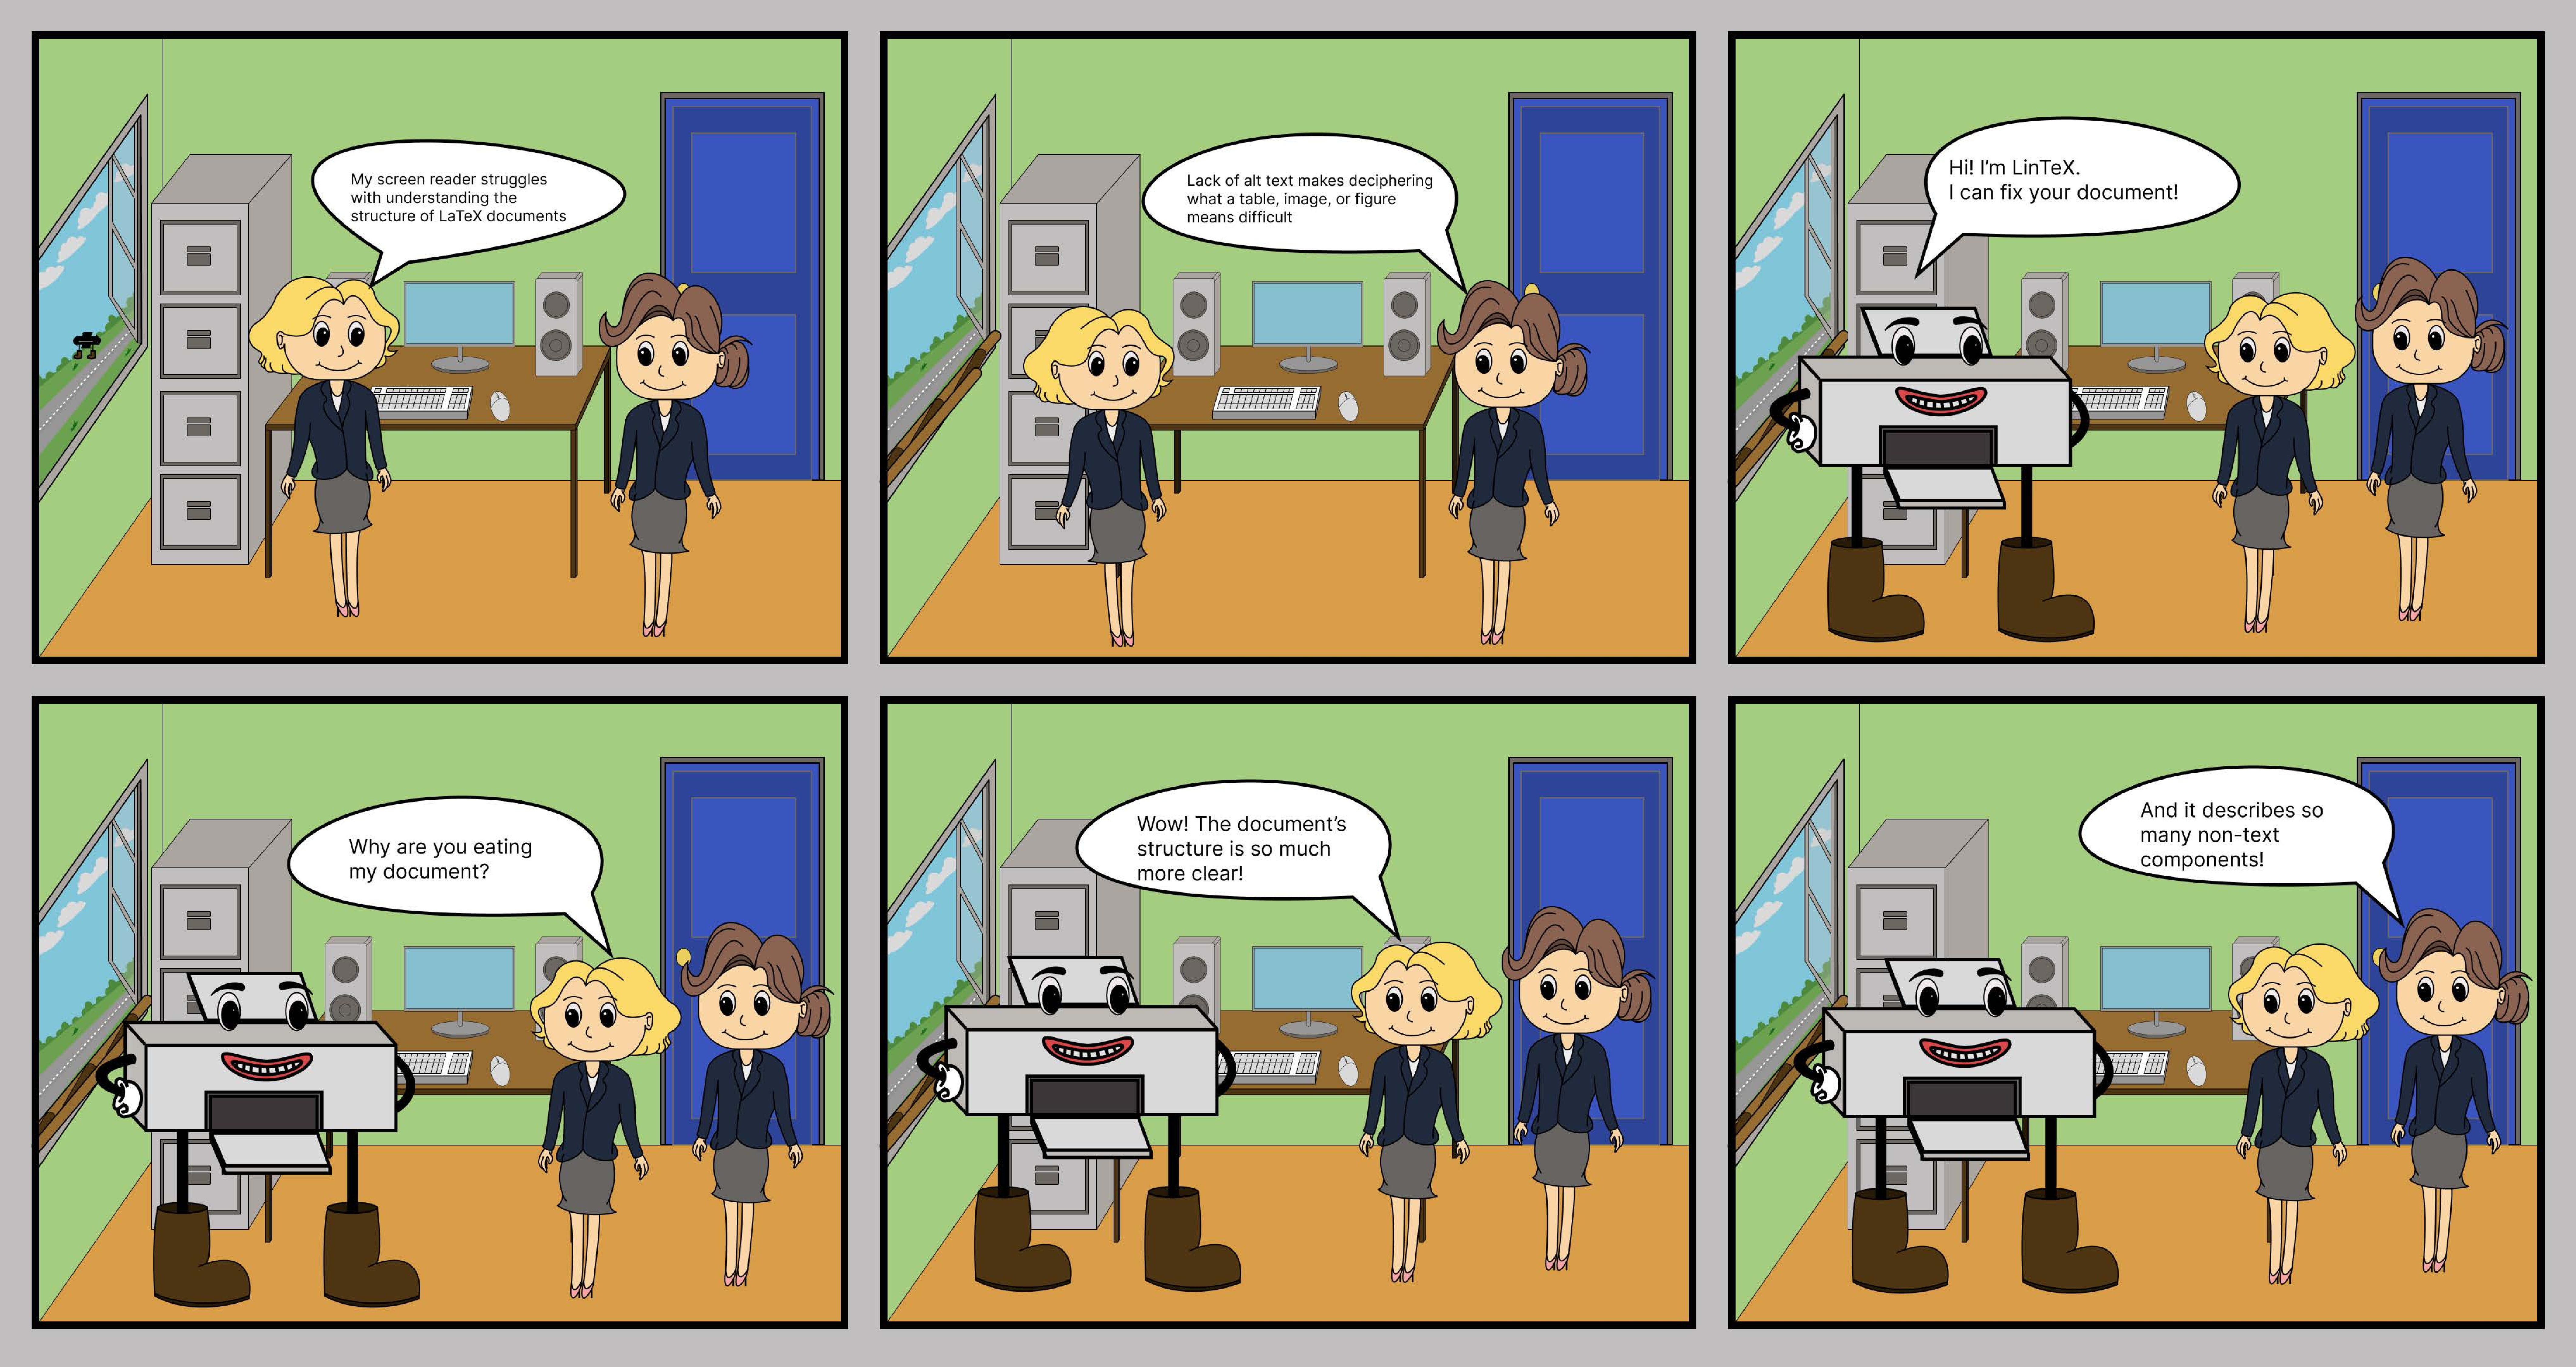
\includepdf[noautoscale=true, width=\paperheight, angle=90]{images/ComicStructure.pdf}
	\clearpage
\end{landscape}

%\input{sections/declaration}
\clearpage
\section*{Acknowledgements}

I would like to thank my supervisor, Brian Mitchell, for his continuous guidance and support throughout the project. His depth of knowledge in related topics and the management of the project overall had vastly improved the project outcome. Although Brian would likely say luck is just a probability taken personally, I consider myself lucky to have come across and taken an interest in his project description.

I would like to provide further thanks to my friends and family who helped provide advice and support throughout the critical periods of the project. Their support was invaluable.

Finally, I would like to give thanks to the anonymous participants who went through the trouble of attending my user study, despite the hassles of it being an in-person session.  % Uncomment to include this page.
\clearpage

%--------------------------------
% Tables of contents.
%--------------------------------
\setstretch{1.0} % 1.0 line spacing.  
\clearpage
\tableofcontents
\listoffigures   % Uncomment for a list of figures.
\listoftables    % Uncomment for a list of tables.
\clearpage

% output glossary
\setglossarystyle{long}
\section{Glossary}
\printglossaries
\clearpage

%--------------------------------
% The body of the document.
%--------------------------------
\pagenumbering{arabic} % Page numbering for rest of document.
\setstretch{1.5} % 1.5 line spacing. 
\section{Introduction}
\subsection{Identifying \LaTeX's key accessibility problems for screen reader users}
Similar to a tool like Microsoft Word, \latexspaced is a tool used to process documents. \latexspaced does this in a programmatical manner, likening it to a programming language, whereas Microsoft Word has a \acrfull{gui} which simplifies the process for an ordinary user. However, \latexspaced prevails in its ability to process scientific documents which may require graphs, images, tables, or advanced mathematical capabilities.

\subsection{Why accessibility is important}


\parencite{accessibility_importance}

- who would benefit from it
        - stats with disabilities e.g. how many people are blind and use screen readers
            - (use good sources e.g. government websites or world health organisations)
        - severity and frequency are considerations
\subsection{Why LuaLaTeX provides better accessibility than PDFLaTeX}
\pdflatexspaced was created to be a media printer, such that it produced PDF documents with the sole purpose of being printed out. Due to its innate design, this means it lacked support for screen reader users. Additionally, as its focus has shifted to maintenance rather than development, \pdflatexspaced is unsuitable for accessibility where requirements change frequently, making it an outdated \texspaced engine.

The introduction of \xetexspaced improved font handling in \latex , yet its lifetime was short-lived, with it being considered an evolutionary deadend, at the addition of \lualatex.

Unlike \pdflatex, \lualatexspaced was created for the purpose of creating electronic documents, giving its development a suitable reason to support screen reader users. Our tool, \lintex, utilises \lualatex's accessibility support, with emphasis placed on screen reader users.

\subsection{Creating LinTeX}
        - intended purpose
        - (this section has the finished overview diagram)
\subsection{aims and objectives}
\subsection{Limitations of the project overall}
\subsection{research questions/hypothesis}


This is a concise and clear overview of your dissertation(more or less 2-3 pages). You can start off the project description provided of the project that was allocated to you and flesh it out.

Include (1) the problem you have tackled, (2) why this problem is worth addressing, (3) what you did to address it - in broad terms. Detail will come later.



i.e., issue(s) on which the research will focus, shall be clearly identified and described. You shall refer to past research work relevant to the topic and objectives, i.e, of the study. You shall outline where applicable the potential research output with respect to research transfer and uptake by the community.

The introduction says: this is an overview of the project. This is why I did it (the problem) and how I tackled it. It is the \emph{runway} into the project. It lets the marker know what to expect of your report.

If you're doing a research project, this would be the place to include the research questions you plan to address. For example:

\begin{description}
\item [RQ1:] Where did James Bond come from?

\item [RQ2:] Why are pumpkins orange?
\end{description}

If you're doing a project of type 1, include a list of objectives. For example:
\begin{description}
\item [Objective 1:] Provide software to allow James Bond to become invisible.

\item [Objective 2:] Provide software to keep track of all loyalty points in one place.
\end{description}

Provide a `map' of your dissertation. For example: Section \ref{backg} reviews the background literature that was reviewed to inform this project. Then Section \ref{process}.....

\subsection{from nov progress}
There is a lack of accessibility with \latex, largely due to usage of outdated PDFLaTeX as opposed to LuaLaTeX. Usage of this outdated TEX engine necessitates workarounds for desired features and accessibility in resulting PDF documents.

\begin{quote}
What can be done to make \latex documents more accessible?
\end{quote}
LinTeX is a developing tool dedicated to combat this problem by focusing on assisting screen readers' abilities to read the PDF documents produced from \latex documents. It aims to cover this area through suggesting structured tagging throughout a document, suggesting components where it may be lacking. Additionally, it will request users to input appropriate alternative text ('alt text') for non-text components of the document, including figures, images, and tables. Further focus may be placed on features such as ensuring appropriate contrast in any colours in the document, appropriate Sans Serif fonts, and flexible document design, largely depending on what development time allows for. 

Additionally, as a tool focused on promoting accessibility, it too should be accessible. Therefore, the tool will ensure strict adherence to the Web Content Accessibility Guidelines 2 (WCAG 2)%~\cite{wcag} requirements with a focus placed on keeping it a simple and intuitive tool for users to make use of.

\begin{quote}
Why should I use LinTeX?
\end{quote}
While the tool is not limited strictly to the field, it is aimed to assist the many academics that find difficulties in accessing reports and academic literatures. By utilising this tool, you can ensure a wider demographic of users can view your documents, without necessitating an especially large amount of research in accessibility; it has been done for you. % Add one file per section.
\clearpage
\input{sections/background-literature} % Add one file per section.
\clearpage
\input{sections/process} % Add one file per section.
\clearpage
\input{sections/product} % Add one file per section.
\clearpage

\input{sections/results} 
\clearpage
\input{sections/reflection} 
\clearpage
\section{Conclusions}\label{conc}
\subsection{Project summary}
\subsection{\nmu Project \nmu limitations}\label{conc:project_limits}
In an ideal world, it would have been possible to have created a project that could target any and all \latexspaced accessibility concerns. Unfortunately, that is outwith the scope of the project, which has been defined as follows:
\begin{itemize}
    \item \lintexspaced is not designed to handle the majority of parsing. Instead, it focuses on a few key elements that are related to the accessibility concerns targetted in our context. Otherwise, it handles a small amount of verification regarding the structure of individual lines and the overall document structure.
    \item This project does not aim to provide automated fixes for errors encountered.
    \item \lintexspaced does not contain an in-built screen reader. While some considerations were put aside for how this could be accomplished, it is not feasible to create an in-built screen reader with the timeframe allocated for this project, due to the vast considerations needed. It might even be a fair statement to consider it a project on its own.
    \item \lintexspaced is not intended to find usage of outdated or incorrect accessibility, but rather to enhance a document's screen reader accessibility through additions to the document.
    \item \lintexspaced is not intended to debug \latexspaced code, as a dedicated \acrfull{ide} and \texspaced engine should be used for this instead.
    \item \lintexspaced expects code to compile in \lualatexspaced before its changes have been applied, with other \texspaced engines being considered outdated and consequently not supported for this context.
    \item \lintexspaced places emphasis on accessibility features for screen reader users.
    \item It is unfeasible to account for all \gls{tagging} options in our context. Therefore, a few key options have been selected based on what would be expected to have the most impact.
\end{itemize}

\subsection{Achievements}


\subsection{Future work}
\lintexspaced has the potential to grow in a variety of manners, such as targetting the limitations in \fullref{conc:project_limits}.

An in-built screen reader for \lintexspaced is an interesting proposition, with it likely being a project by itself due to the lack of finer details requiring vast amounts of consideration and the difficulties with finding similar materials, seeing as most references for an in-built screen reader appear to point to screen readers as a browser extension. However, it may be possible to make \lintexspaced work with those extensions to provide the ideal experience for the end user.

Automated fixes, with the addition of being able to fix several identical errors at once, would be a great feature to include in \lintex . There is potential for this feature to work alongside the error handling of \lintex , yet this has unfortunately not been explored further at this time.

Additionally, highlighting why \lintexspaced has recommended a change would make the experience a lot more insightful and better encourage developers to be inclusive of screen reader users in the future.

Finally, utilising HTMX to make \lintexspaced more responsive to the end user's actions would allow for a more immersive experience for the user, while keeping the technologies required at a reasonable minimum requirements.
\subsection{Reflection}


\subsection{Final thoughts}


%--------------------------------
% Bibliography
%--------------------------------
\clearpage
\setstretch{1.0}  % 1.0 line spacing. 
\bibliographystyle{abbrv}
\bibliography{bibliography}
% add references to the file called bibliography.bib
\clearpage

%--------------------------------
% Appendices
%--------------------------------
\appendix
\setstretch{1.5} % 1.5 line spacing.
\section{Appendix}
\subsection{\nmu Ethical \nmu approval}\label{appendix:ethics_approval}
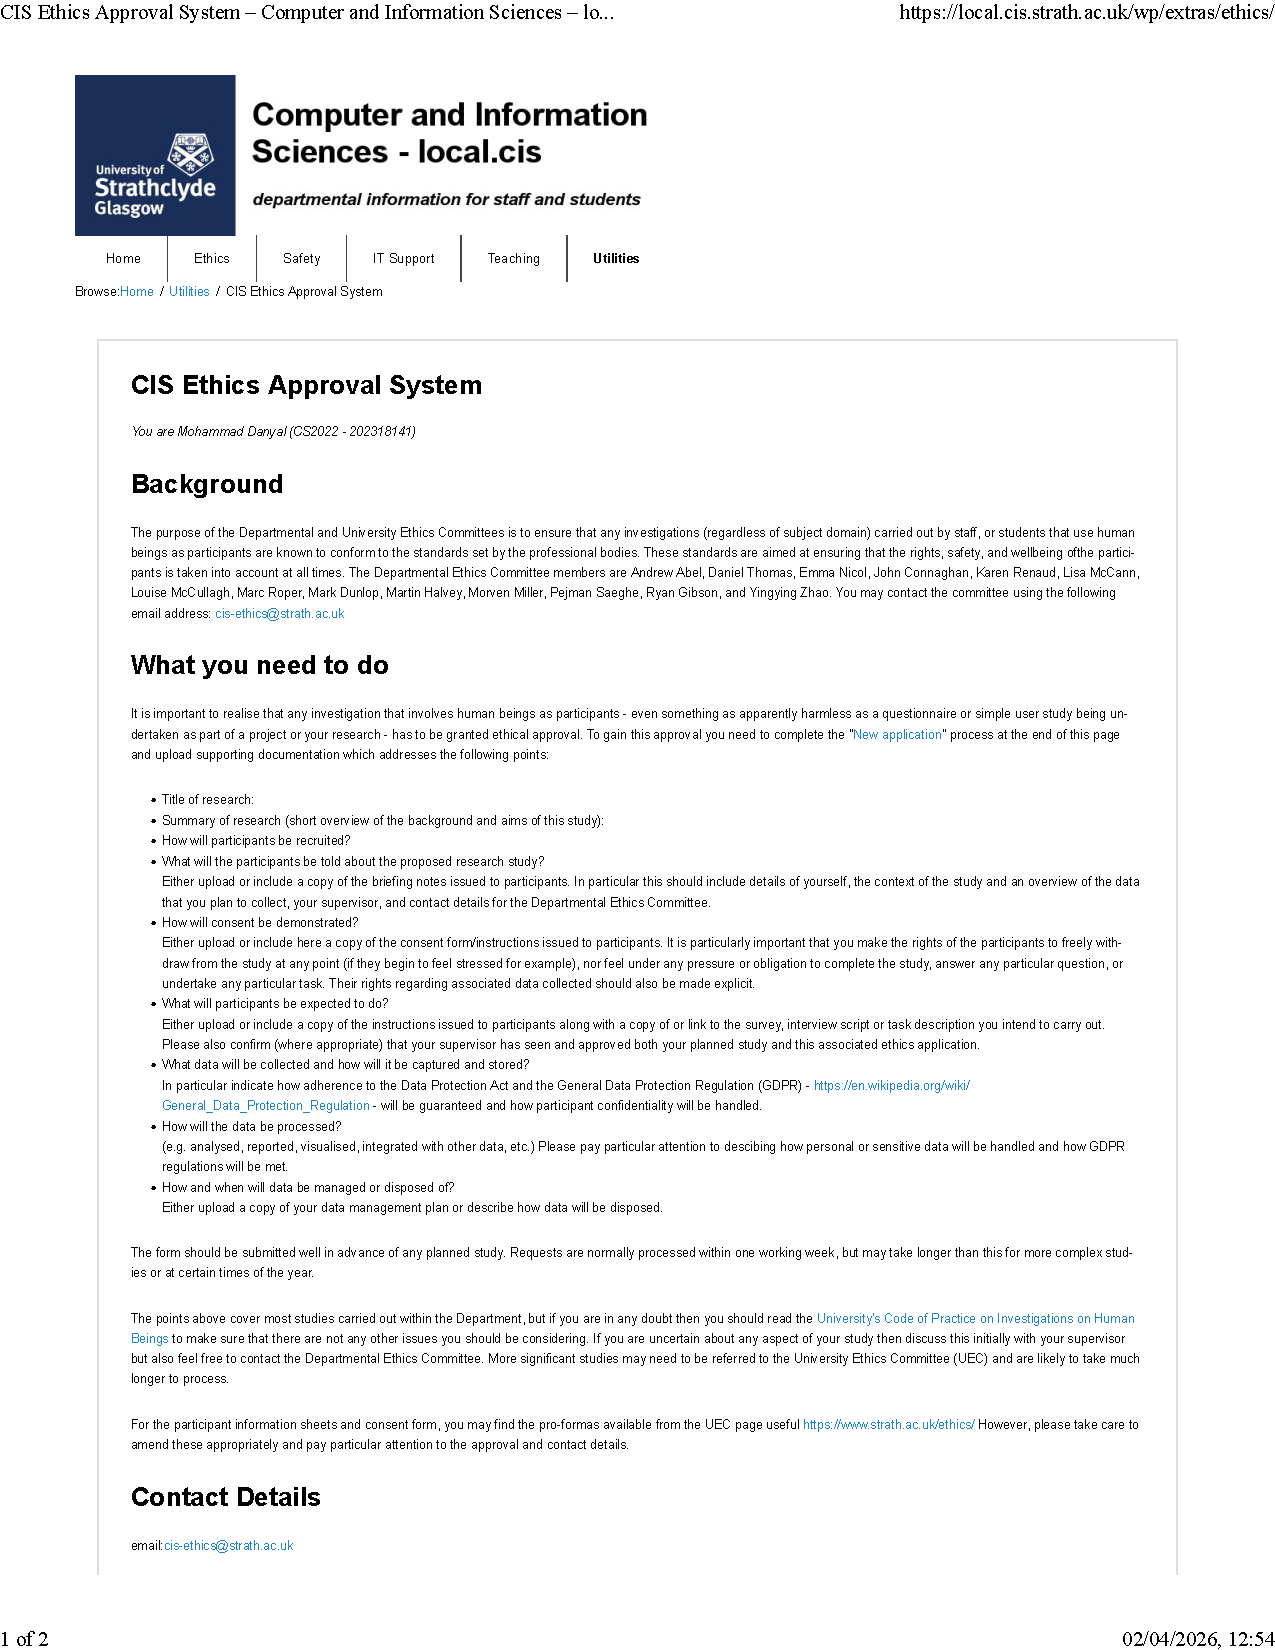
\includepdf[pages=-]{images/ethics_approval}

\subsection{Ethics application}
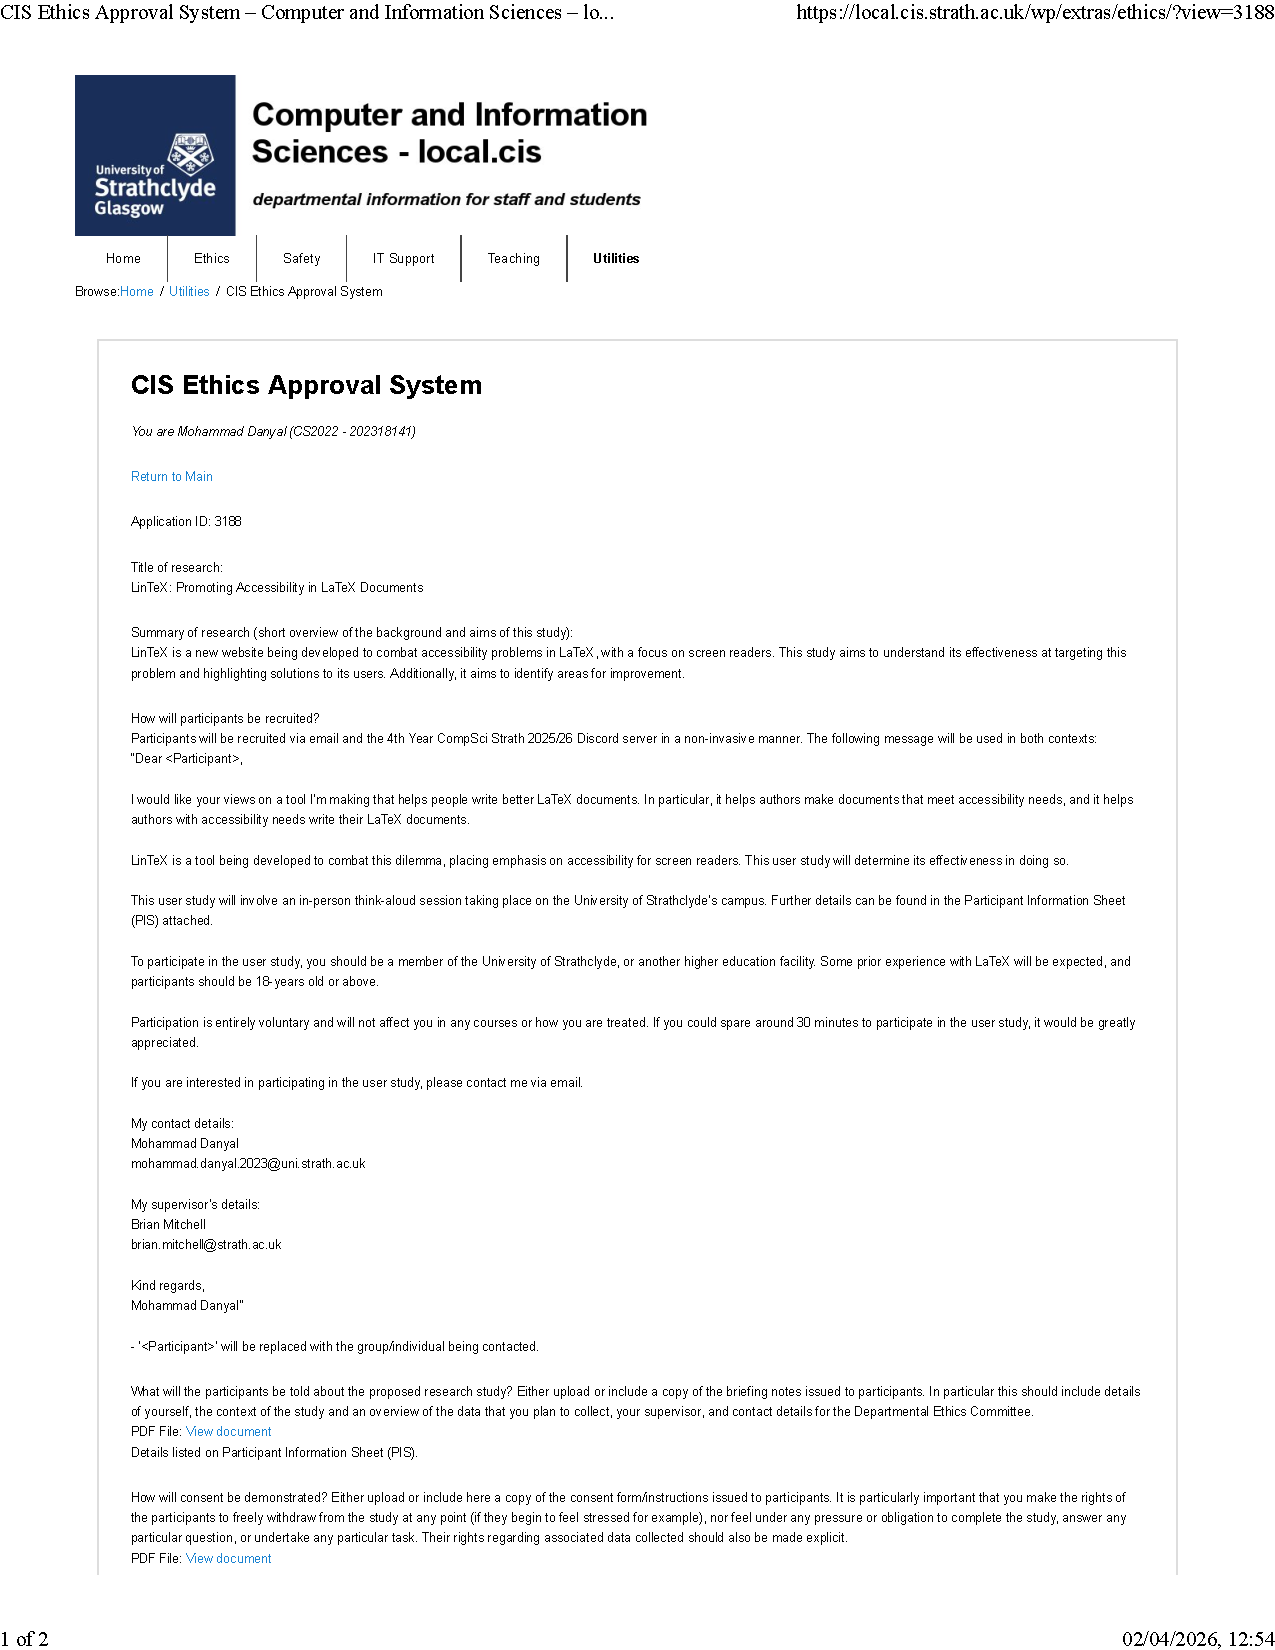
\includepdf[pages=-]{images/ethics_application}

\subsection{Participant information sheet}
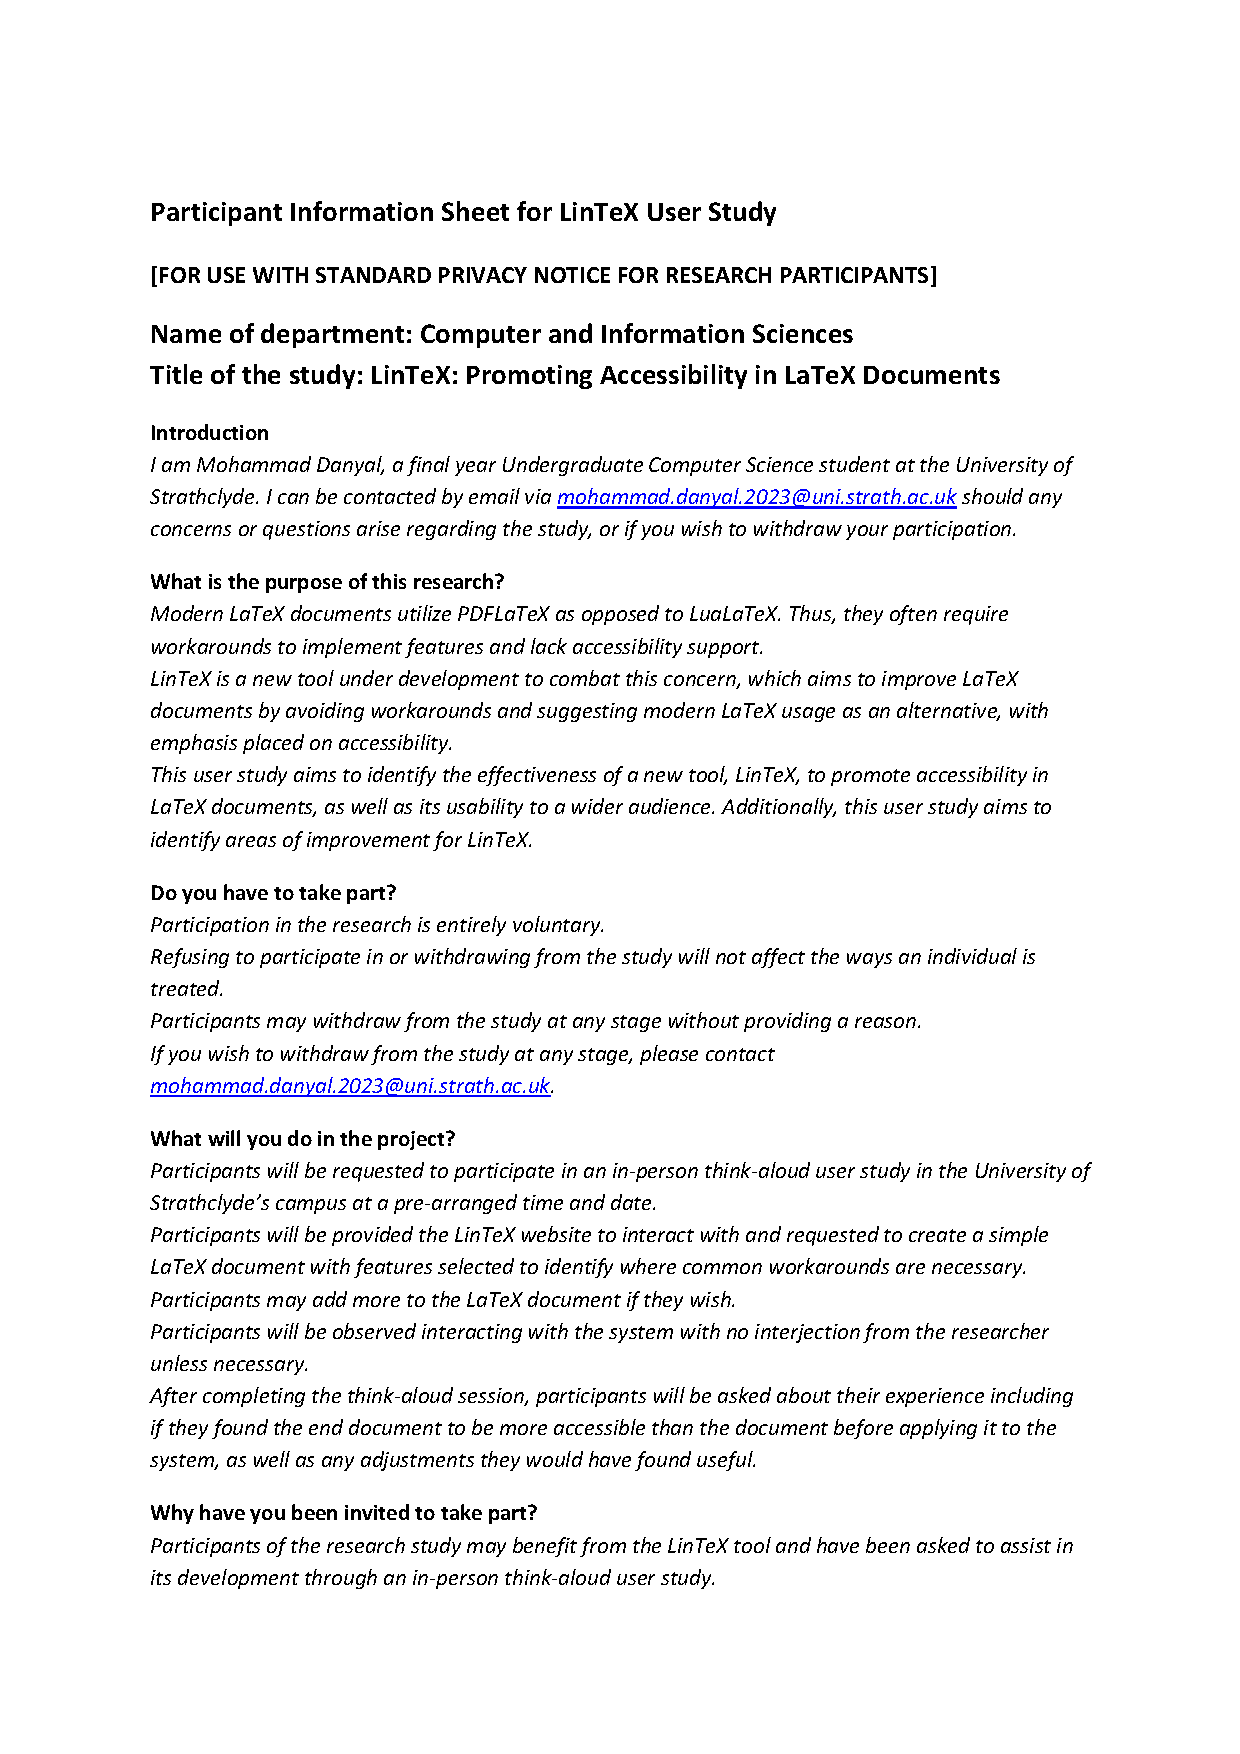
\includepdf[pages=-]{images/participant_info_sheet}

\subsection{Consent form}
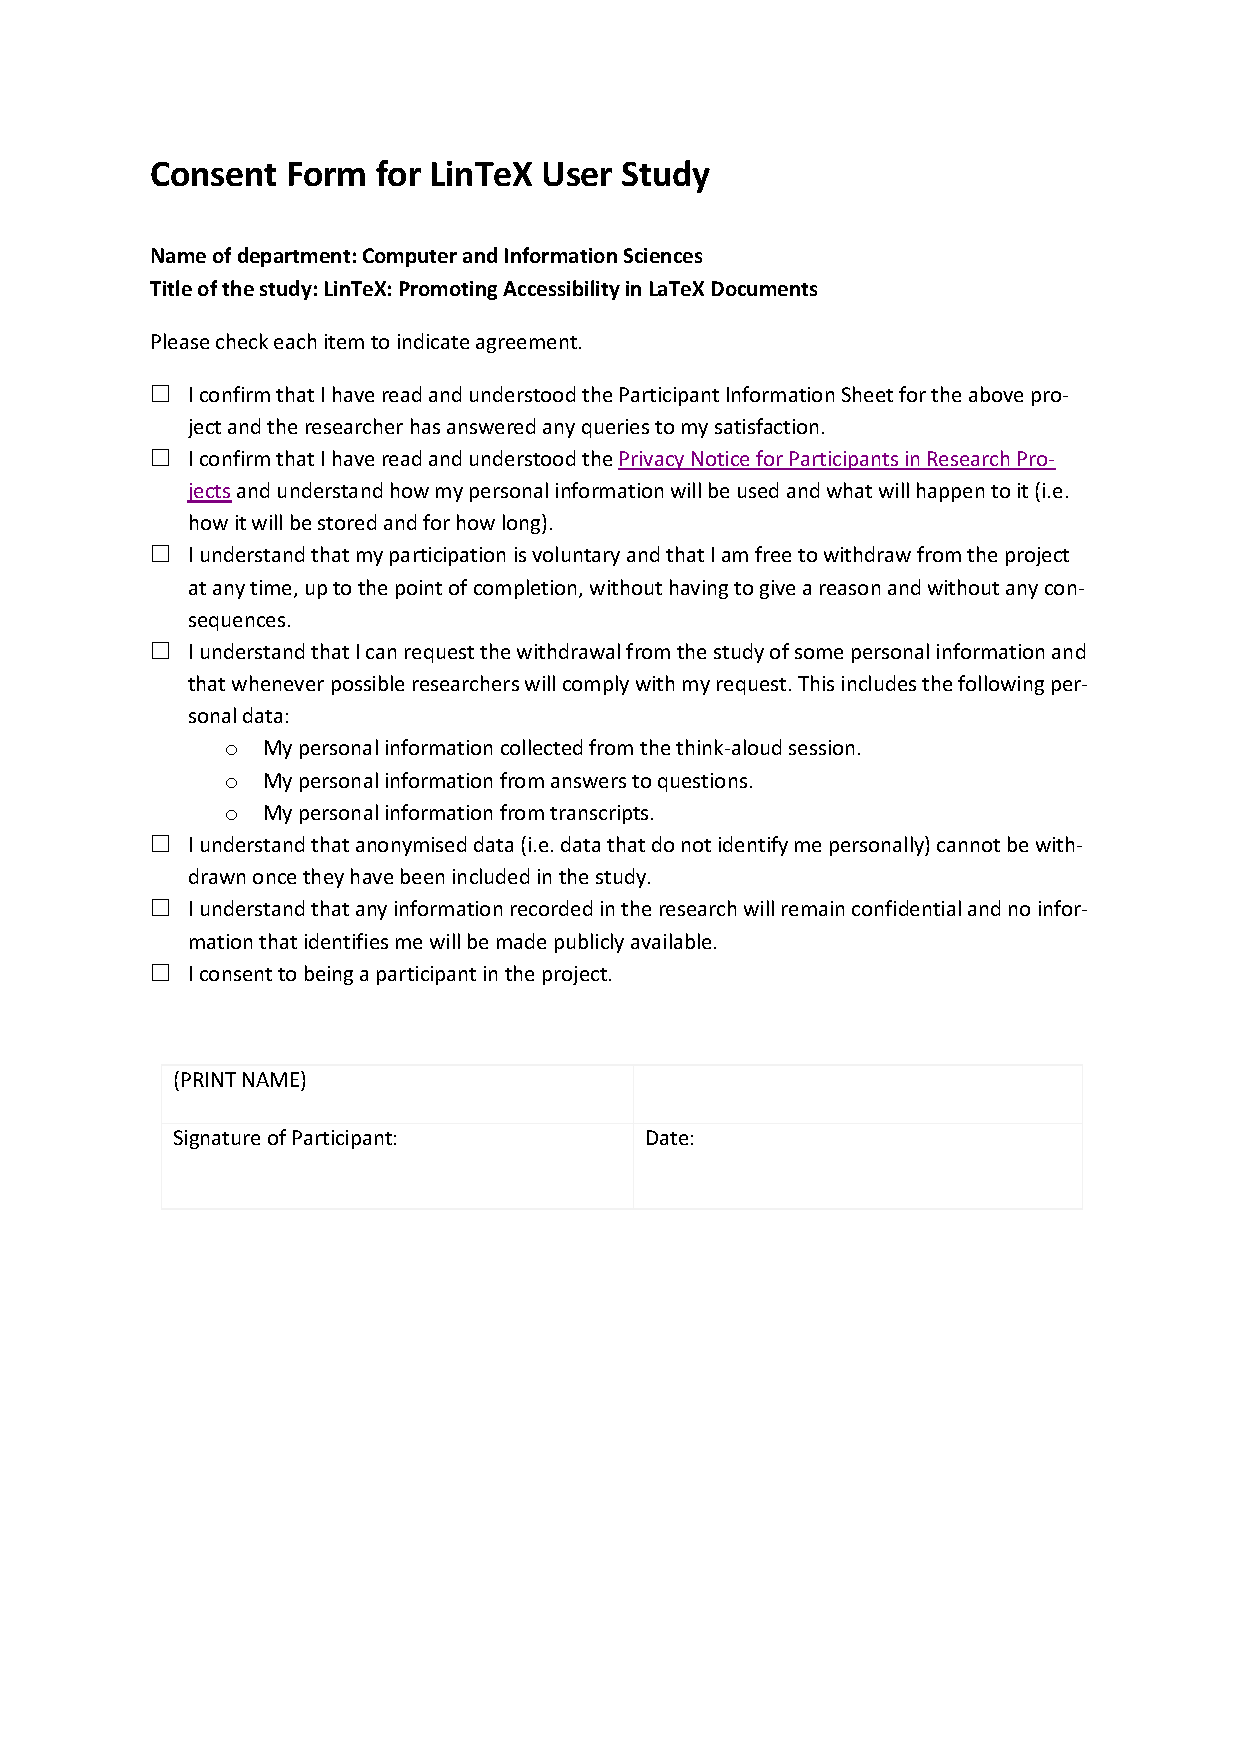
\includepdf[pages=-]{images/consent_form}

\subsection{\nmu User \nmu study script}\label{appendix:user_study_script}
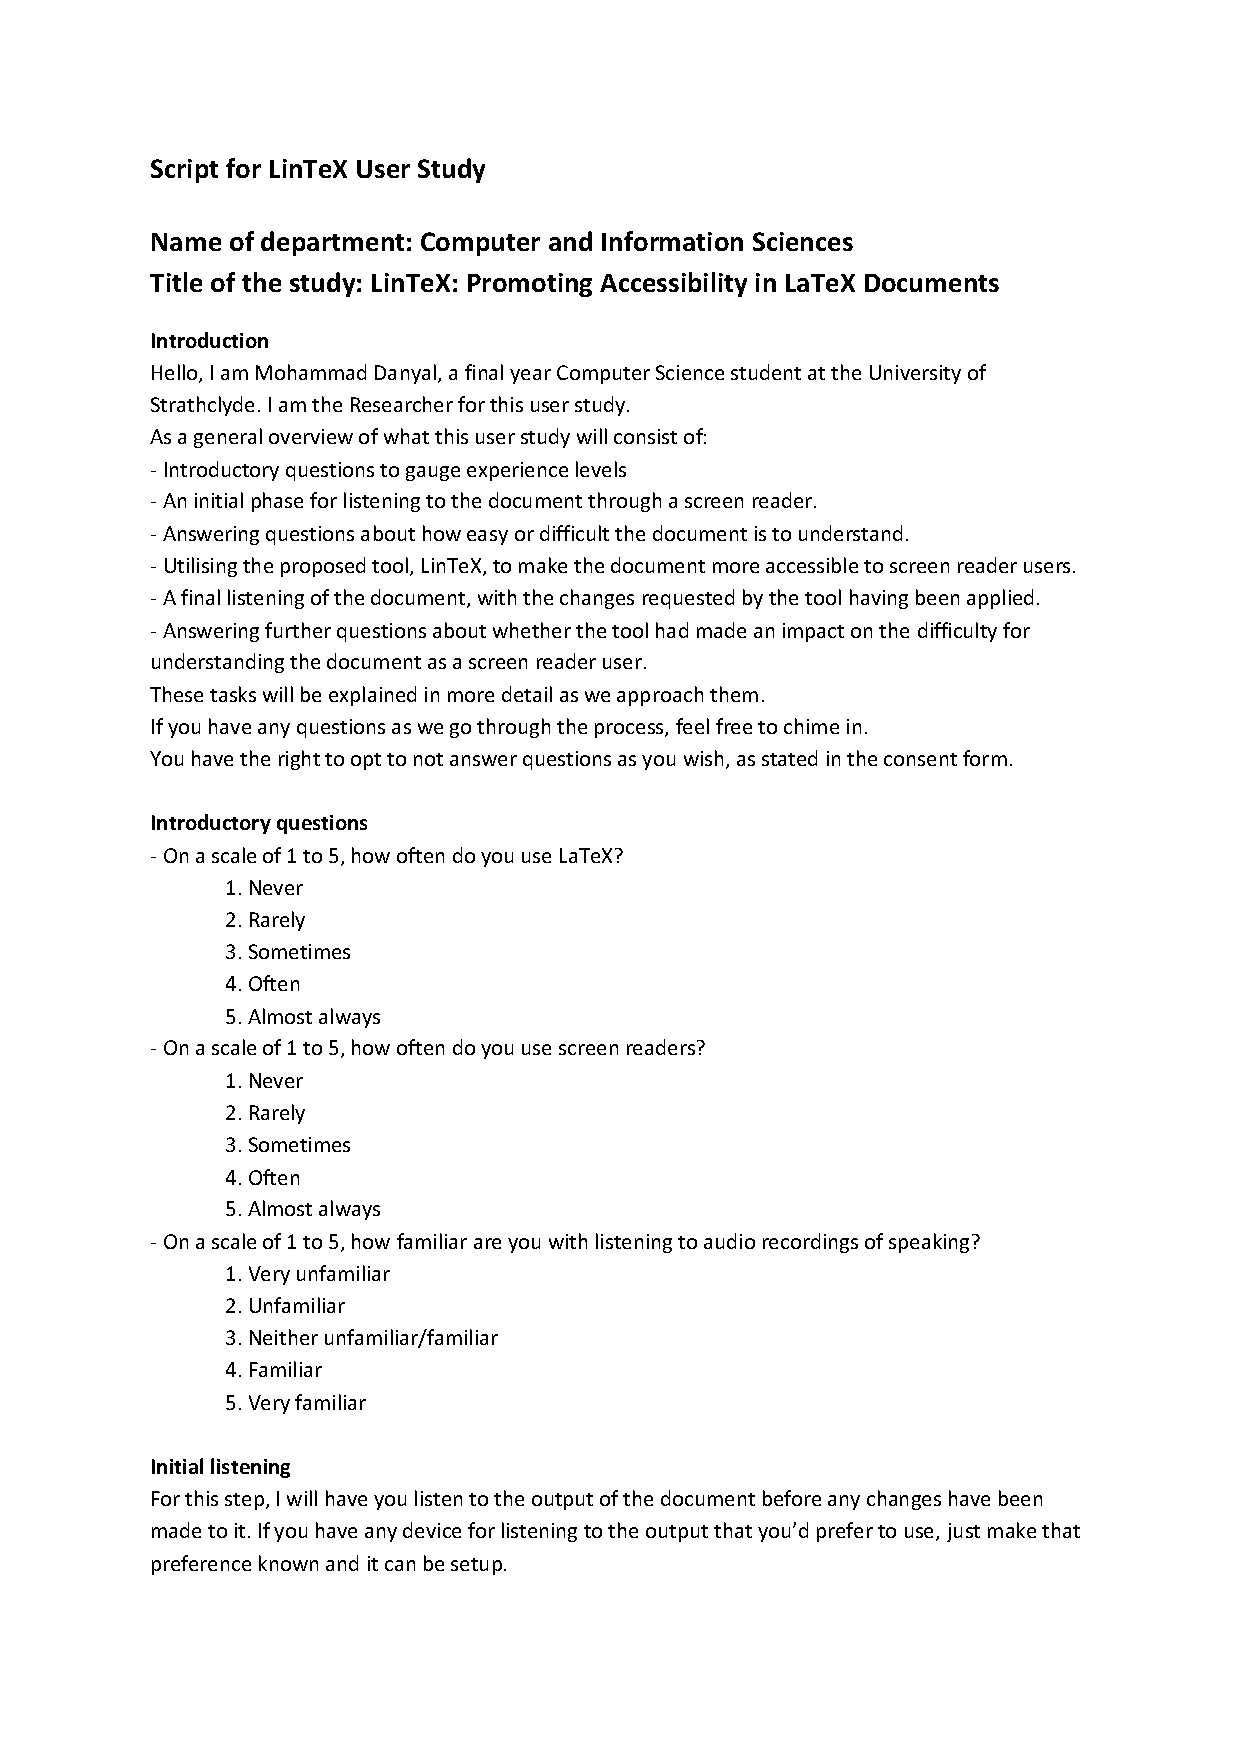
\includepdf[pages=-]{images/user_study_script}

\subsection{\Gls{inaccessible_doc}}\label{appendix:inaccessible_doc}
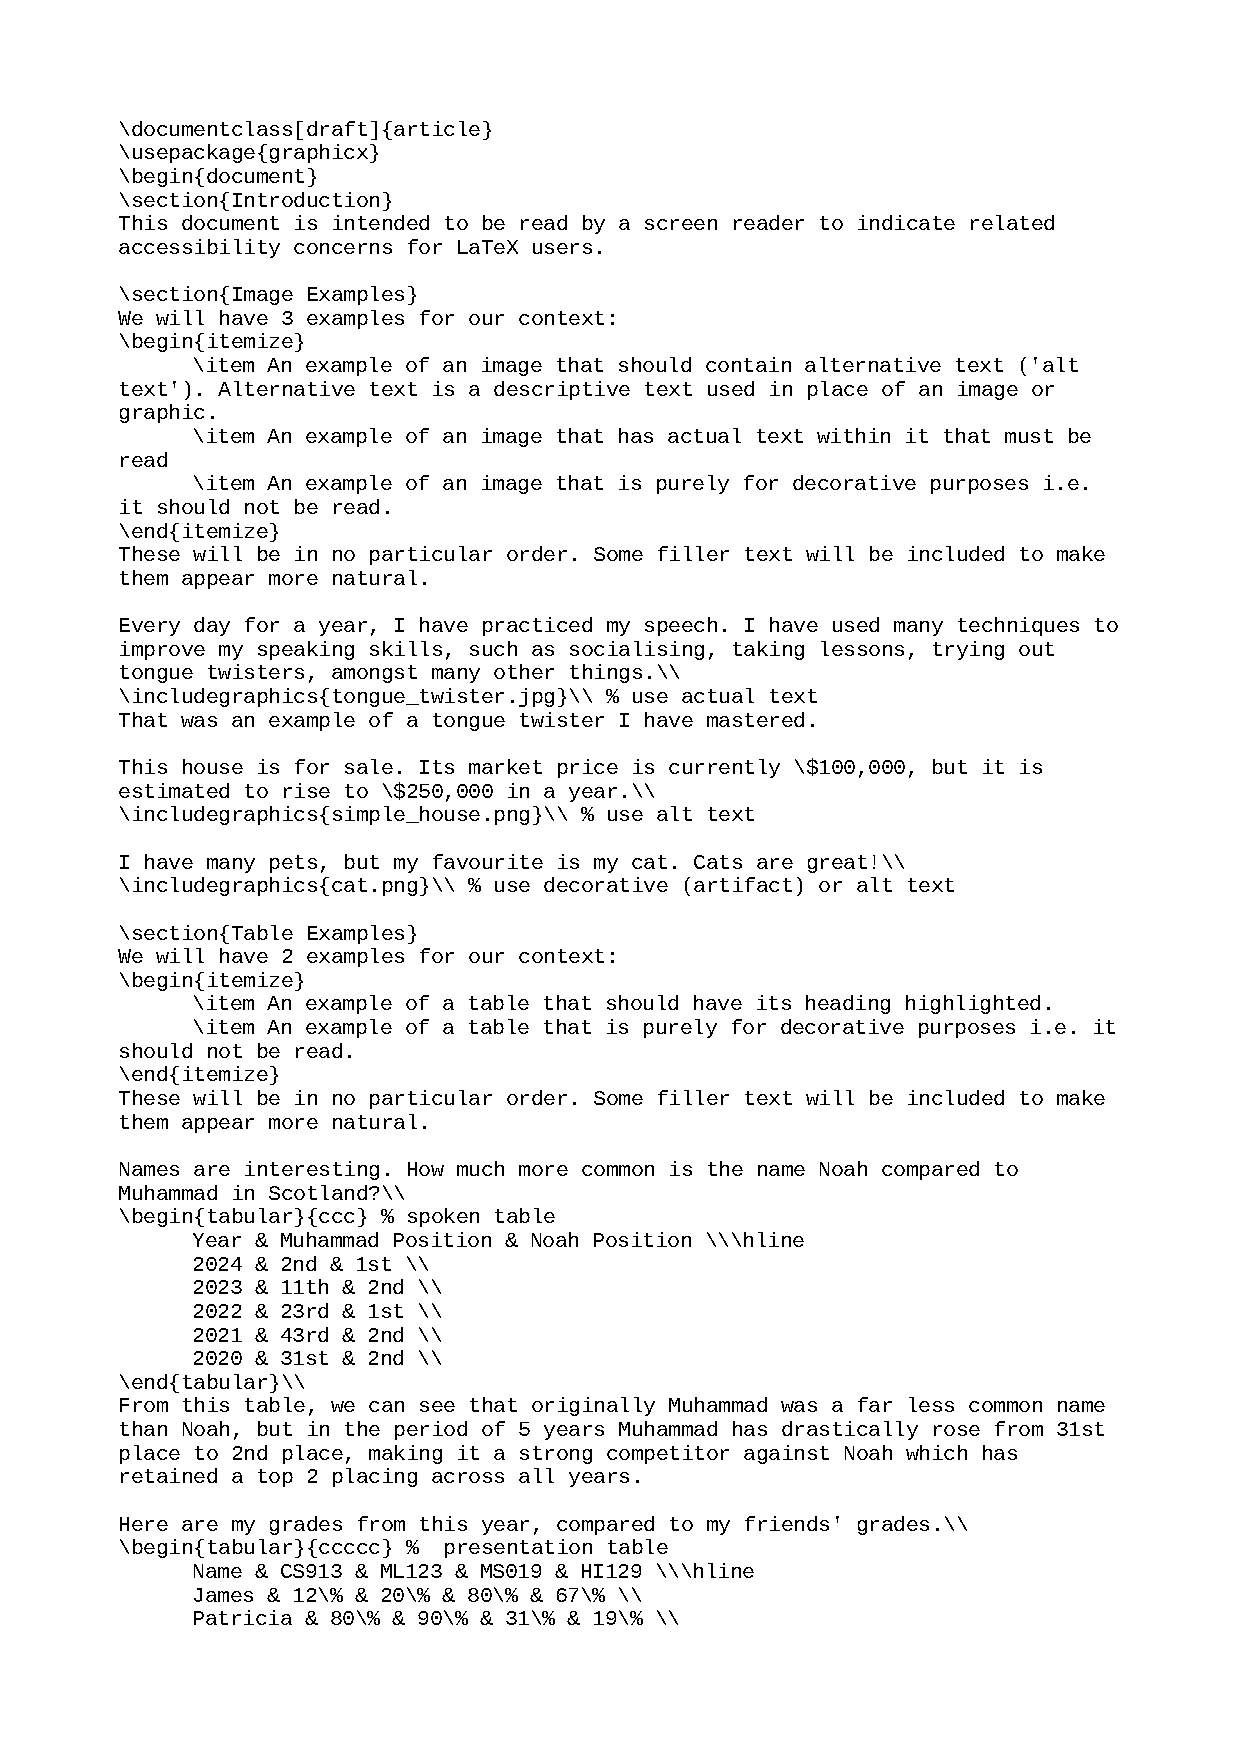
\includepdf[pages=-]{images/inaccessible_document}

\subsection{\Gls{accessible_doc}}\label{appendix:accessible_doc}
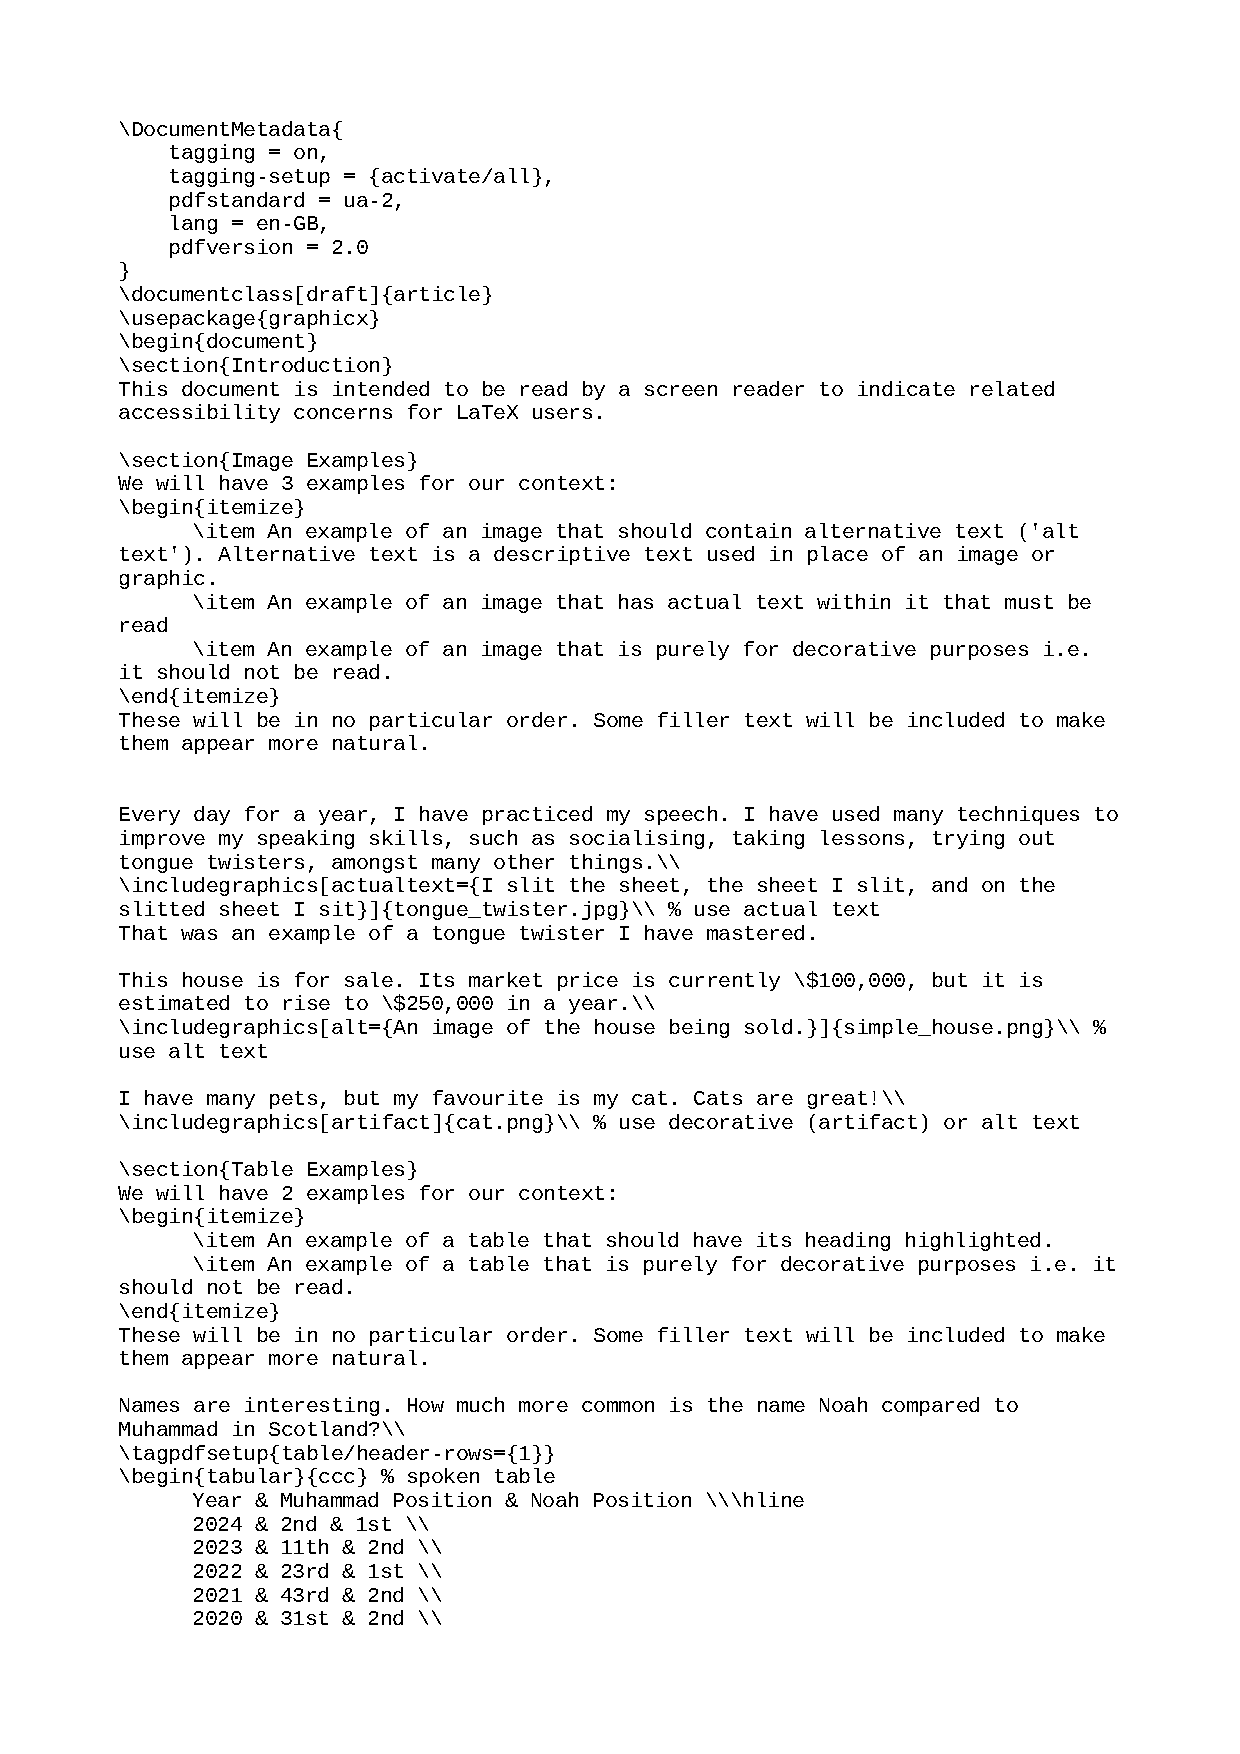
\includepdf[pages=-]{images/accessible_document}

\subsection{\acrshort{peg} script}\label{appendix:peg_script}
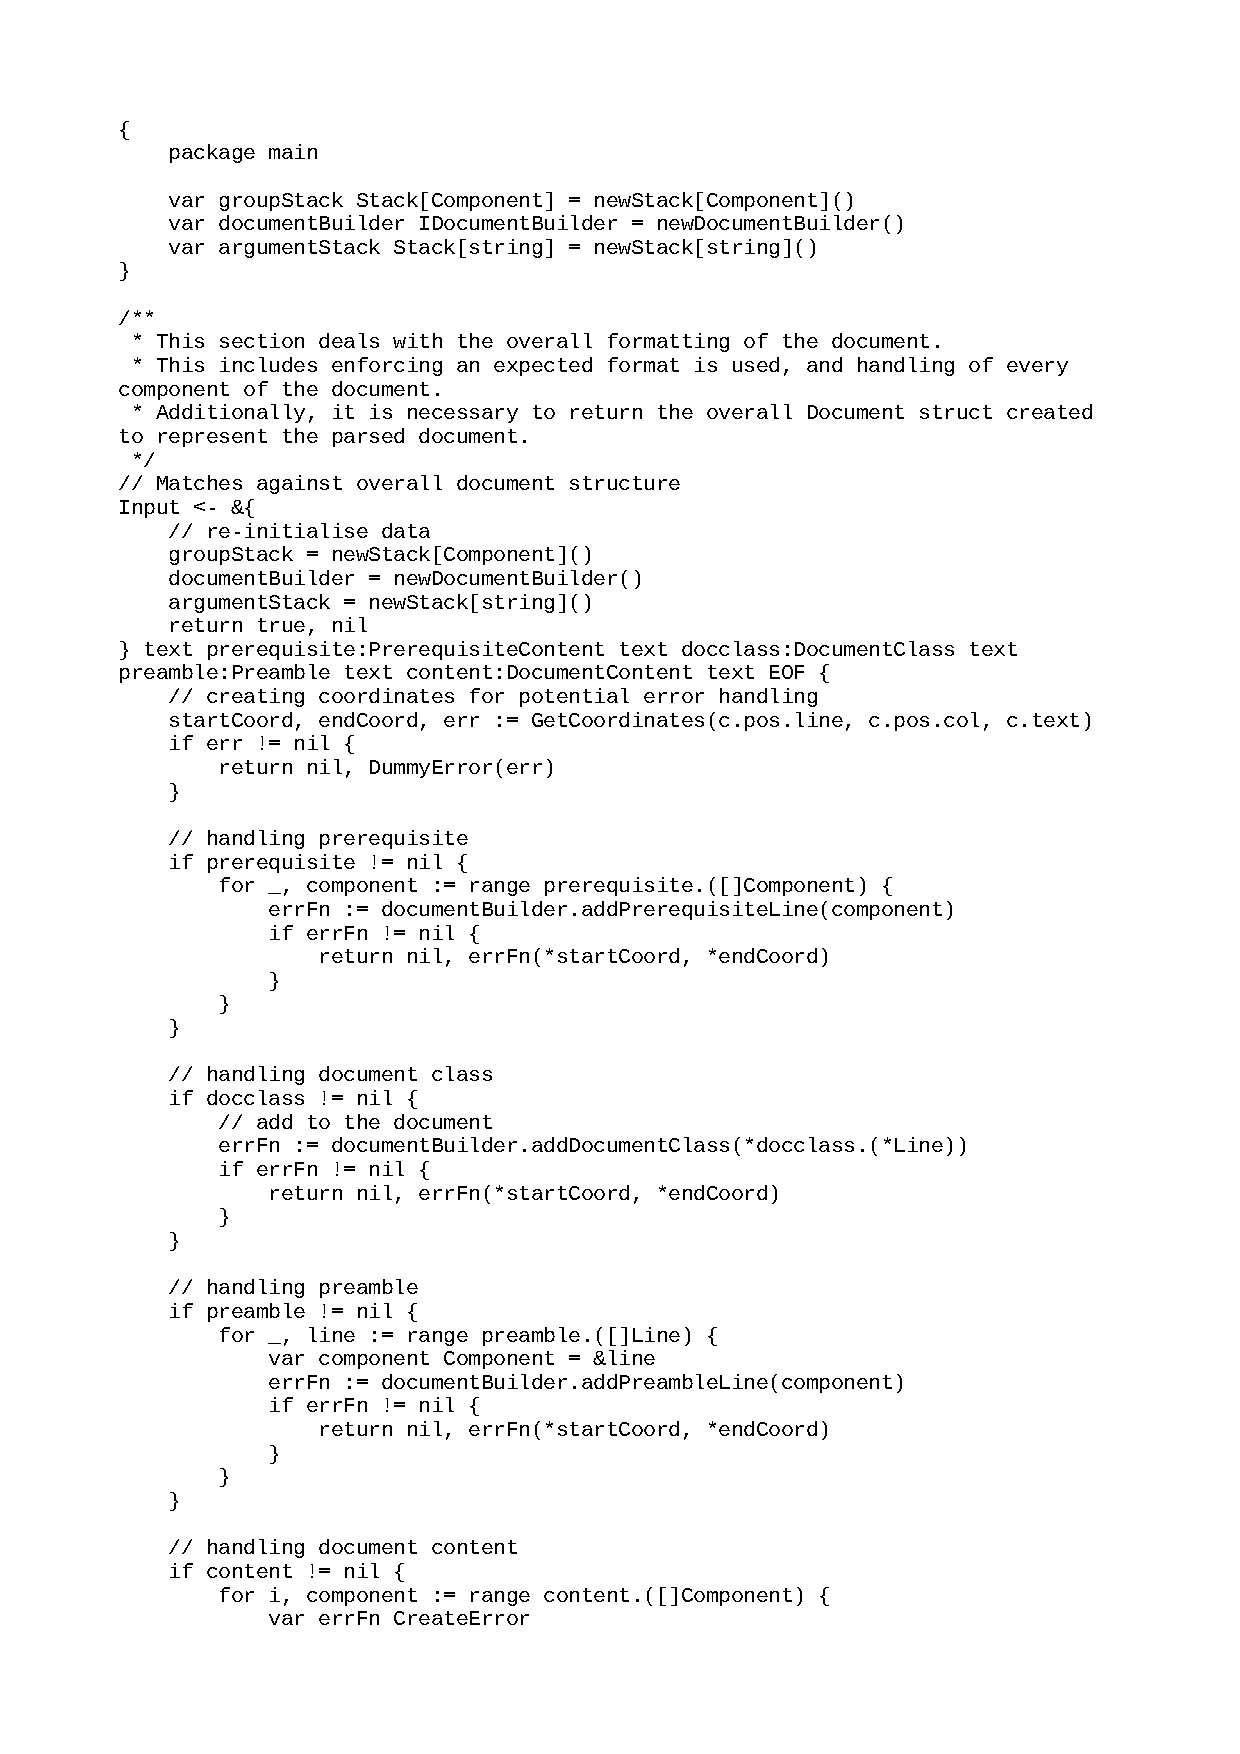
\includepdf[pages=-]{images/peg_script}

\clearpage % Add one file per appendix

\end{document}